\documentclass[11pt]{report}
%\usepackage{fancybox}
\usepackage{geometry}
\usepackage{amsmath}
\usepackage{txfonts}
\usepackage{layout}
\usepackage{setspace}
%\usepackage{mathptmx}
\geometry{a4paper, left=22mm, right=22mm, top=25mm, bottom=25mm}
\usepackage{wrapfig}
\usepackage[dvipdfm]{graphicx,hyperref}
\usepackage{mediabb}
\setstretch{1.3}
\title{\Huge\bf{Role of Noncollective Excitations in Low-Energy Heavy-Ion Fusion Reaction
and Quasi-Elastic Scattering}}
\author{\\\\\\\\\\\\\\\\\\\\\\\\\\\\{\it\Large Department of Physics, Faculty of Science, Tohoku University}\\\\
\Huge Shusaku Yusa}
\date{March, 2013}
\begin{document}


\chapter{Noncollective excitations in $^{20}$Ne + $^{90,92}$Zr reaction}
In this chapter, we investigate the role of noncollective excitations in the
quasi-elastic scattering for $^{20}$Ne + $^{90,92}$Zr systems.
We employ the random matrix model to describe the noncollective excitation in
coupled-channels calculation.
The effect on the quasi-elastic barrier distribution is discussed.

\section{Quasi-elastic scattering for $^{20}$Ne + $^{90,92}$Zr systems}
For $^{20}$Ne + $^{90,92}$Zr systems, quasi-elastic scattering experiments were
performed at energies around the Coulomb barrier\cite{piasecki}.
From the measured quasi-elastic scattering cross sections,
the quasi-elastic barrier
distribution has been extracted,
as has been shown in Fig. \ref{fig1.2}.
The obtained quasi-elastic scattering barrier distributions show a different
behavior between the two systems, that is, the barrier distribution for $^{20}$Ne +
$^{92}$Zr is much more smeared compared to that of $^{20}$Ne + $^{90}$Zr system.
The dashed line in Fig.\ref{fig1.2}(a) shows the barrier distribution
obtained with a
coupled-channels calculation which takes into account the
collective excitations of $^{20}$Ne and $^{90}$Zr, that is, the rotational
excitations of $^{20}$Ne and the vibrational excitations of $^{90}$Zr.
The calculation reproduces the peak structure of the barrier distribution,
while it yields somewhat broader separation of the
peaks, which is probably due to the treatment of separation vector in nuclear
potential\cite{BB82, H73}.
On the other hand,
the calculated barrier distribution for the $^{20}$Ne +
$^{92}$Zr system shows the similar behavior to that of 
the $^{20}$Ne + $^{90}$Zr system, and does not exhibit a smeared behavior 
observed in the experimental barrier distribution.
This similarity in the barrier distributions of the two systems
is because the deformation of 
$^{20}$Ne is so large that the difference in the vibrational excitations of Zr
isotopes plays a minor role for the barrier distribution.
Thus, the conventional coupled-channels calculation cannot
reproduce the barrier distribution for both the systems simultaneously.

As has been discussed in Chap. 1,
the difference in the barrier distributions
between the two systems has been conjectured
to arise from noncollective excitations that are not taken into account
explicitly in the coupled-channels calculations.
In this chapter, we take into account the noncollective excitations of Zr
isotopes in the calculations for $^{20}$Ne + $^{90,92}$Zr reactions
and see whether the difference in
the quasi-elastic barrier distributions can be explained by the 
noncollective excitations.
See Fig. \ref{fig1.3} for the energy spectra for the Zr isotopes.


\section{Random matrix model}
In the previous chapter, we investigated the effects of the noncollective
excitations in $^{16}$O + $^{208}$Pb reaction.
In that calculation, the description of the noncollective excitations is based
on the experimental information of the noncollective states.
Especially, the deformation parameter $\beta_{\lambda}$, which 
gives the transition
strength to the noncollective states,
has been experimentally known for most of low-lying noncollective states
in $^{208}$Pb.
For $^{90,92}$Zr, however, the information on the deformation parameter is
rather limited compared to that for $^{208}$Pb.
That is, even though the energy and the spin are experimentally known
for many noncollective states\cite{bnl},
basically nothing is known for the coupling strength to the ground
state.
Therefore, one has to resort to a different approach to describe the
noncollective excitations in $^{20}$Ne + $^{90,92}$Zr reactions.
For this purpose, we employ the random matrix model discussed in
Sec. 4.5.
In this model, we consider the ensemble of the coupling matrix elements
and assume the ensemble to make a
gaussian orthogonal ensemble(GOE) in the random matrix theory.
This model was originally applied to the calculations for deep inelastic
collisions by Weidenm\"uller and his collaborators in the
1970's\cite{KPW76, AKW78, akw1,akw2,akw3,akw4}.
We show in appendix B an application of the random matrix model to a 
one-dimensional barrier penetration problem.
The work presented in this chapter
can be considered as an extension of this
one-dimensional problem
to a three-dimensional realistic problem.

We construct the coupling matrix for the noncollective states
as follows.
The coupling Hamiltonian is expanded in multipoles as
\begin{eqnarray}
V_{\rm coup}({\bvec{r}}, {\bvec{\xi}}) = \sum_{\lambda}F_{\lambda}({\bvec{r}})
\cdot T_{\lambda}(\bvec{\xi}),
\end{eqnarray}
with
\begin{eqnarray}
  \left\{
    \begin{array}{c}
      F_{\lambda\mu}({\bvec{r}}) = f_{\lambda}(r)Y_{\lambda\mu}(\hat{\bvec{r}}) \\
      T_{\lambda\mu}({\bvec{\xi}}) =
                  t_{\lambda}\left(\xi\right)Y_{\lambda\mu}(\hat{\bvec{\xi}}).
    \end{array}
  \right.
\end{eqnarray}
Then, the coupling Hamiltonian
in the iso-centrifugal approximation is obtained by transforming
to the rotating frame as
\begin{eqnarray}
V_{\rm coup}(r, {\bvec{\xi}}) 
= \sum_{\lambda} f_{\lambda}(r)Y_{\lambda}^*(\hat{\bvec{r}}=0)\cdot
  T_{\lambda}(\bvec{\xi})
= \sum_{\lambda}\sqrt{\frac{2\lambda+1}{4\pi}} f_{\lambda}(r)T_{\lambda 0}(\bvec{\xi}).
\end{eqnarray}
Using the Wigner-Eckart theorem, the coupling matrix element reads
\begin{eqnarray}
V_{nn^\prime}^{II^{\prime}}(r) &=& \langle \phi_{nI} | V_{\rm coup}(r) |
\phi_{n^{\prime}I^{\prime}} \rangle  \nonumber \\
&=& \sum_{\lambda}\sqrt{\frac{4\pi}{2\lambda+1}} (-1)^I
  \left(
    \begin{array}{ccc}
      I & \lambda & I^\prime \\
      0 & 0 & 0
    \end{array}
  \right)
  \langle nI || V_\lambda(r) Y_{\lambda}|| n^\prime I ^\prime \rangle
\end{eqnarray}
with
\begin{eqnarray}
V_{\lambda}(r,\xi) = \frac{2\lambda+1}{4\pi} f_{\lambda}(r)t_{\lambda}(\xi).
\end{eqnarray}
Following Weidenm\"uller {\it et al.},
we introduce here the statistical assumption of GOE.
That is, we require that the ensemble average 
of the coupling matrix element vanishes, i.e.,
\begin{eqnarray}
\overline{V_{nn^\prime}^{II^\prime}(r)} = 0. \label{goe_1}
\end{eqnarray}
We also require the reduced matrix elements to satisfy the following equation
\begin{eqnarray}
& &\overline{
\langle nI || V_{\lambda}(r) Y_{\lambda} || n^{\prime}I^{\prime} \rangle
\langle n^{\prime\prime}I^{\prime\prime} || V_{\lambda^{\prime}}(r^{\prime}) Y_{\lambda^{\prime}} || n^{\prime\prime\prime}I^{\prime\prime\prime} \rangle
} \nonumber \\
&=& \sqrt{(2I+1)(2I^\prime+1)} \frac{2\lambda+1}{4\pi}
   \left\{\delta_{nn^{\prime\prime}}\delta_{n^{\prime}n^{\prime\prime\prime}} 
          \delta_{II^{\prime\prime}}\delta_{I^{\prime}I^{\prime\prime\prime}}
   + (-1)^{I-I^\prime}\delta_{nn^{\prime\prime\prime}}\delta_{n^{\prime}{n^{\prime\prime}}}
                      \delta_{II^{\prime\prime\prime}}\delta_{I^{\prime}{I^{\prime\prime}}}
   \right\}  \nonumber\\
   & &\times\  \delta_{\lambda\lambda^\prime} 
\alpha_{\lambda}(n,n^\prime;I,I^\prime;r, r^\prime),
\end{eqnarray}
or, in terms of the coupling matrix elements, we require
\begin{eqnarray}
\overline{V_{nn^\prime}^{II^\prime}(r)V_{n^{\prime\prime}n^{\prime\prime\prime}}^{I^{\prime\prime}I^{\prime\prime\prime}}(r^\prime)}
&=& \left\{\delta_{nn^{\prime\prime}}\delta_{n^{\prime}n^{\prime\prime\prime}} 
          \delta_{II^{\prime\prime}}\delta_{I^{\prime}I^{\prime\prime\prime}}
   + \delta_{nn^{\prime\prime\prime}}\delta_{n^{\prime}{n^{\prime\prime}}}
                      \delta_{II^{\prime\prime\prime}}\delta_{I^{\prime}{I^{\prime\prime}}}
   \right\}
   \sqrt{(2I+1)(2I^\prime+1)} \\ \nonumber
& & \times \sum_{\lambda}
   \left(
     \begin{array}{ccc}
       I & \lambda & I^{\prime} \\
       0 & 0 & 0
     \end{array}
   \right)^{2}
\alpha_{\lambda}(n,n^\prime;I,I^\prime;r, r^\prime).
\label{goe_2}
\end{eqnarray}
Here, the form factor $\alpha_{\lambda}$ is given by
\begin{eqnarray}
\alpha_{\lambda}(n,n^\prime;I,I^\prime;r, r^\prime) =
\frac{w_\lambda}{\sqrt{\rho(n,I)\rho(n^\prime,I^\prime)}}
e^{-\frac{(\epsilon_n-\epsilon_n^\prime)^2}{2\Delta^2}}
e^{-\frac{(r-r^{\prime})^2}{2\sigma^2}}
h(r)h(r^{\prime}),
\label{form_factor_org}
\end{eqnarray}
where $\rho(n,I)$ is a level density with spin $I$ at excitation energy
$\epsilon_n$, $h(r)$ is a some function of $r$, and
($w_{\lambda}, \Delta, \sigma$) are parameters.
The level density in the denominator
of the form factor reflects the complexity of the
noncollective states,
as we have discussed in Sec. 4.5.
We present in appendix C the calculation method of the coupling matrix elements.
Concerning the coupling to the noncollective excitations,
we consider only the coupling from the ground state.
Therefore, one of the level densities entered in the form factor is
constant in our calculations.
Thus we modify the form factor as
\begin{eqnarray}
\alpha_{\lambda}(n,0;I,0;r, r^\prime) =
\frac{w_\lambda}{\sqrt{\rho(n)}}
e^{-\frac{\epsilon_n^2}{2\Delta^2}}
e^{-\frac{(r-r^{\prime})^2}{2\sigma^2}}
h(r)h(r^{\prime}),
\label{form_factor}
\end{eqnarray}
where, 0 means the ground state.
We have also replaced the spin dependent level density by the total
level density for the sake of simplicity.

Before applying the model to the reaction of $^{20}$Ne + $^{90,92}$Zr systems,
we first apply the model to $^{16}$O + $^{208}$Pb system
in order to study the validity of the model by 
comparing the results with the
more reliable results which
use the experimental information on the noncollective
states as presented in the previous section.



\section{Level density and strength distribution}
In order to apply the random matrix model to $^{16}$O + $^{208}$Pb,
we first discuss the treatment of the level density $\rho(n)$.
The level density is defined by
\begin{eqnarray}
\rho(\epsilon) = \sum_n \delta(\epsilon -\epsilon_n),
\end{eqnarray}
which is a discrete spectrum.
From this discrete spectrum, we define a continuous level density,
which is used
in the calculation of the coupling matrix elements
in the random matrix model.
To do this, we first define the following function
\begin{eqnarray}
N(\epsilon) =  \int^\epsilon_0 \rho(\epsilon^\prime)d\epsilon^\prime.
\label{num_levels}
\end{eqnarray}
This gives the number of levels up to the excitation energy $\epsilon$.
We fit $N(\epsilon)$ with a polynomial function.
In Fig. \ref{fig7.5}, we show the fitting result for $^{208}$Pb nucleus.
We use the $N(\epsilon)$ in the interval between 4 MeV and 7.5 MeV
and fitted with a polynomial
$\displaystyle f(\epsilon) = \sum_{n=0}^6 a_n\epsilon^n$.
\begin{figure}[t]
  \center
  \begin{minipage}[t]{78mm}
    \includegraphics[clip,keepaspectratio,width=78mm]{figure/chapter7/level_fit.eps}
    \caption{The number of levels of $^{208}$Pb 
    up to the excitation energy $\epsilon$
    as a function of $\epsilon$. The dots
    represents experimental data and the red line is a fitting
    function.}
    \label{fig7.5}
  \end{minipage}
  \hspace{0.5cm}
  \begin{minipage}[t]{78mm}
    \includegraphics[clip,keepaspectratio,width=78mm]{figure/chapter7/level_density.eps}
    \caption{Continuous level density obtained as a first derivative
             of the fitting function $f(\epsilon)$
             shown in Fig.\ref{fig7.5}.}
    \label{fig7.6}
  \end{minipage}
\end{figure}
The resultant values of $a_n$ are
$a_0=-7479, a_1=6969$ (MeV$^{-1}$), $a_2=-2612$ (MeV$^{-2}$),
$a_3=497.5$ (MeV$^{-3}$), $a_4=-49.59$ (MeV$^{-4}$),
$a_5=2.347$ (MeV$^{-5}$), and $a_6=-0.03632$ (MeV$^{-6}$).
The continuous level density is then defined by the first derivative of
$f(\epsilon)$, that is, $df(\epsilon)/d\epsilon$,
which is shown in Fig. \ref{fig7.6}.

Using this level density, we calculate the strength distribution which we
define by (see Eqs. (\ref{goe_2}) and (\ref{form_factor}))
\begin{eqnarray}
b_I = 
\sqrt{
\sum_{\lambda}
  \left(
    \begin{array}{ccc}
      0 & \lambda & I \\
      0 & 0 & 0
    \end{array}
  \right)^2
  \sqrt{\frac{2I+1}{\rho(\epsilon)}}
  e^{-\frac{\epsilon^2}{2\Delta^2}}
  \label{strength_dist}
}
\end{eqnarray}
($w_{\lambda}$ is omitted in the definition by assuming $w_{\lambda} = w$ for
all ${\lambda}$).
This quantity corresponds to the distribution of the deformation parameter
$\beta_{I}$, since, in the linear coupling approximation, the coupling
matrix elements are given by
\begin{eqnarray}
V_{0n}(r) = - \beta_I R_{\rm T}\frac{dV_{\rm N}}{dr}.
\end{eqnarray}
\begin{figure}[t]
\center
  \includegraphics[clip,keepaspectratio,width=120mm]{figure/chapter7/strength_dist.eps}
  \caption{Transition strength distributions for $^{208}$Pb 
  as a function of excitation energy $\epsilon$.
  The black line is the distribution of the experimental 
  deformation parameters and the red line
  is the strength distribution defined in Eq. (\ref{strength_dist}) with RMT.
  Both distributions are smeared with a gaussian function with a width of 0.15 MeV.
  The black line is scaled by a factor of 10.}
  \label{fig7.7}
\end{figure}  
Fig.\ref{fig7.7} shows a comparison of experimental deformation parameter,
$\beta_I$, and the strength distribution in RMT, $b_I$, as a function of
excitation energy. The parameter $\Delta$ in (\ref{strength_dist}) is chosen to
be 7 MeV.
Both distributions are smeared with a gaussian function whose width is 0.15 MeV.
The deformation parameter is scaled by a factor of 10 because the dimension of
$\beta_I$ and $b_I$ is not taken to be the same, while the both quantities 
determine the coupling strength to each excited state.
Although the small deficiency of the strength 
can be seen for peaks between 5.5 MeV and 7 MeV,
the overall peak structure of the strength distribution is reasonably
reproduced by the random matrix model. 

\section{Test of random matrix model with $^{16}$O + $^{208}$Pb reaction}
In this section, we apply the random matrix model to $^{16}$O + $^{208}$Pb
reaction in order to see whether the random matrix model works well for the
description of the noncollective excitations
in low-energy heavy-ion reactions.

For the function $h(r)$ in the form factor (\ref{form_factor}), we adopt the
following form
\begin{eqnarray}
h(r) = \frac{e^{(r-R_n)/a}}
{\left[1 + e^{(r-R_n)/a}\right]^2},
\end{eqnarray}
which is the same functional form 
as the derivative of the Woods Saxon potential.
Thus, the coupling matrix elements become similar to that of the vibrational
coupling in the linear coupling approximation.
For the parameters in Eq. (\ref{form_factor}), we use $w = 38000$ MeV$^{3/2}$,
$\Delta = 7$ MeV, and $\sigma = $4.0 fm. The value of $\Delta$ is chosen so that
all the considered excited states up to 7.382 MeV have a chance to be excited.
The values of $\Delta$ and $\sigma$ are the same as those used in Refs.
\cite{akw3,akw4}. The value of $w$ is chosen so that the random matrix model
reproduces the results obtained with the experimental $\beta_I$.
\begin{figure}[t]
\center
  \includegraphics[clip,keepaspectratio,width=85mm]{figure/chapter7/fus_16O_208Pb_WS_linear.eps}
  \caption{The fusion cross sections((a) and (b)) and
  the fusion barrier
  distributions((c)) for $^{16}$O + $^{208}$Pb system.
  The red lines are the results obtained with the experimental
  deformation parameter. The blue lines are the results of the calculation based on
  the random matrix model.
  The black dashed lines are the results of the calculation with
  only the collective excitations.}
  \label{fig7.8}
\end{figure}

In Fig.\ref{fig7.8}, we show the comparison for fusion cross sections.
The potential has the same geometry as that used in the previous chapter, 
while the potential depth is set to be 550 MeV, because
in these calculation, we do not take into account the excitation of $^{16}$O
for simplicity.
The red lines show the results using the experimental deformation parameters.
This calculation is similar to that in the previous chapter, while the linear
coupling approximation is employed in the present calculation.
The blue lines are the results using the random matrix model for the description
of the noncollective excitations.
For comparison, the calculation which takes into account only the collective
excitations are show by the black dashed lines.
By choosing an appropriate parameter $w$, we can see that the random matrix
model nicely reproduces the results which use the experimental deformation
parameters.
Therefore, we conclude that the random matrix model is applicable to the 
description of the noncollective excitations by choosing appropriate parameters
in the model.



\section{Application to $^{20}$Ne + $^{90,92}$Zr systems}
\subsection{Parameters}
Encouraged by the comparative study presented in the previous section,
we now apply the random matrix model to the $^{20}$Ne + $^{90,92}$Zr reactions.
We use the same parameters as those used in Ref.\cite{piasecki}, that is,
the surface diffuseness parameter of $a = 0.63$ fm, the radius parameter of $r_0 =
1.2$ fm, and the potential depth parameter of $V_0 = 59.9$ MeV.
For this potential, the height of the 
Coulomb barrier becomes $V_{\rm B} = 51.76$ MeV.

As for the coupling to $^{20}$Ne, we take into account the rotational
states in the ground band up to $6^+$ state with the deformation parameters
$\beta_2 = 0.46$ and $\beta_4 = 0.27$.
The octupole phonon state at 5.62 MeV is also considered with $\beta_3 = 0.39$.
For the coupling to collective states in $^{90}$Zr nucleus, we take into
account the vibrational $2^+$ state at 2.18 MeV with $\beta_2=0.089$ and
$3^-$ state at 2.75 MeV with $\beta_3 = 0.211$\cite{KMM10}.
For $^{92}$Zr, we take into account the vibrational $2^+$ state at 0.93 MeV with
$\beta_2^{({\rm N})} = 0.144$ and $\beta_2^{({\rm C})} = 0.103$ as well as $3^-$
state at 2.34 MeV with $\beta_3 = 0.17$\cite{NMD01}. These phonon excitations in Zr isotopes
are taken into account up to the two-phonon state, while the mutual excitations of
quadrupole and octupole phonon states are not included.
\begin{figure}[t]
  \center
  \begin{minipage}[t]{78mm}
    \includegraphics[clip,keepaspectratio,width=78mm]{figure/chapter7/level_fit_90Zr.eps}
    \caption{Same as Fig. \ref{fig7.5}, but for $^{90}$Zr.}
    \label{level_fit_90Zr}
  \end{minipage}
  \hspace{0.5cm}
  \begin{minipage}[t]{78mm}
    \includegraphics[clip,keepaspectratio,width=78mm]{figure/chapter7/level_density_90Zr.eps}
    \caption{Same as Fig. \ref{fig7.6}, but for $^{90}$Zr.}
    \label{ld_90Zr}
  \end{minipage}
\end{figure}
\begin{figure}[h]
  \center
  \begin{minipage}[t]{78mm}
    \includegraphics[clip,keepaspectratio,width=78mm]{figure/chapter7/level_fit_92Zr.eps}
    \caption{Same as Fig. \ref{fig7.5}, but for $^{92}$Zr.}
    \label{level_fit_92Zr}
  \end{minipage}
  \hspace{0.5cm}
  \begin{minipage}[t]{78mm}
    \includegraphics[clip,keepaspectratio,width=78mm]{figure/chapter7/level_density_92Zr.eps}
    \caption{Same as Fig. \ref{fig7.6}, but for $^{92}$Zr.}
    \label{ld_92Zr}
  \end{minipage}
\end{figure}

For the coupling to the noncollective states,
we use the experimental data for the excitation energies and spins.
The coupling matrix elements themselves are calculated by the random matrix model.
Among the noncollective states, we take into account only the
natural parity states, because the unnatural parity states are not probable to be
excited compared to the natural parity states in the collision of even-even nuclei.
The noncollective states are assumed to be coupled
only to the ground state for
simplicity, which corresponds to the linear coupling approximation.
For the parameters in the random matrix model, we employ $\Delta=7$ MeV,
$\sigma=4$ fm, and $w = 200$ MeV$^{3/2}$.
The values of $\Delta$ and $\sigma$ are the same as in the calculations for
$^{16}$O + $^{208}$Pb reaction, and the value of $w$ is determined so that the
calculated barrier distribution for the $^{20}$Ne + $^{92}$Zr system
agrees with the experimental barrier distribution
as well as possible.
\begin{figure}[h]
  \center
  \begin{minipage}[t]{78mm}
    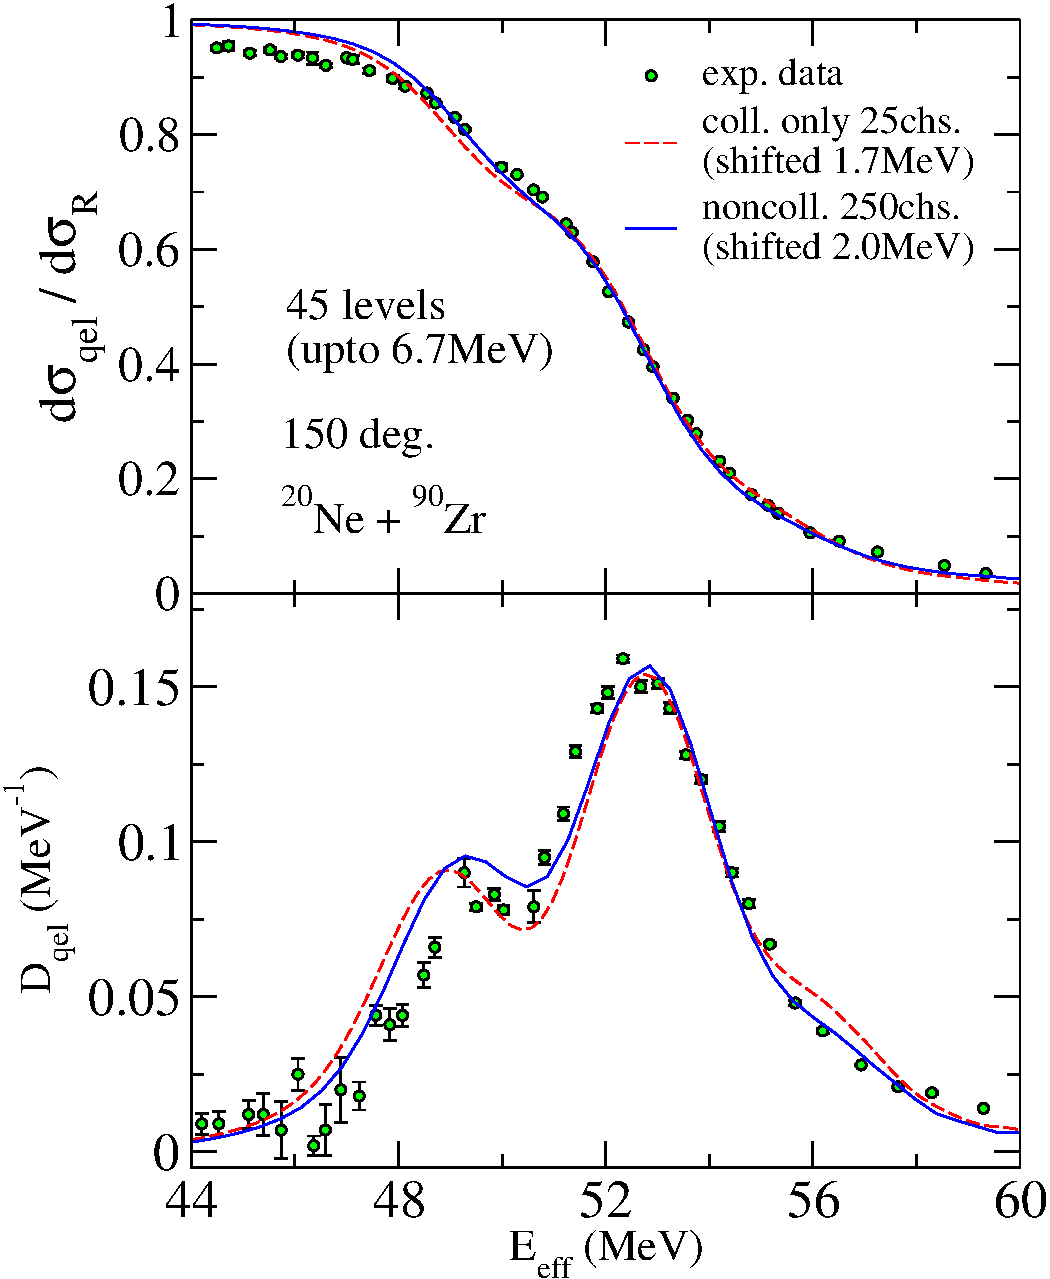
\includegraphics[clip,keepaspectratio,width=78mm]{figure/chapter7/qel_20Ne_90Zr_150deg_noncoll_w0_200.pdf}
    \caption{Quasi-elastic cross sections (upper panel) and quasi-elastic
    barrier distribution (lower panel) for $^{20}$Ne + $^{90}$Zr system at 150$^{\circ}$.
    The red dashed lines are the results with only the collective excitations, while
    the blue lines are the results which include the noncollective excitations in
    addition to the collective excitations.}
    \label{fig7.9}
  \end{minipage}
  \hspace{0.5cm}
  \begin{minipage}[t]{78mm}
    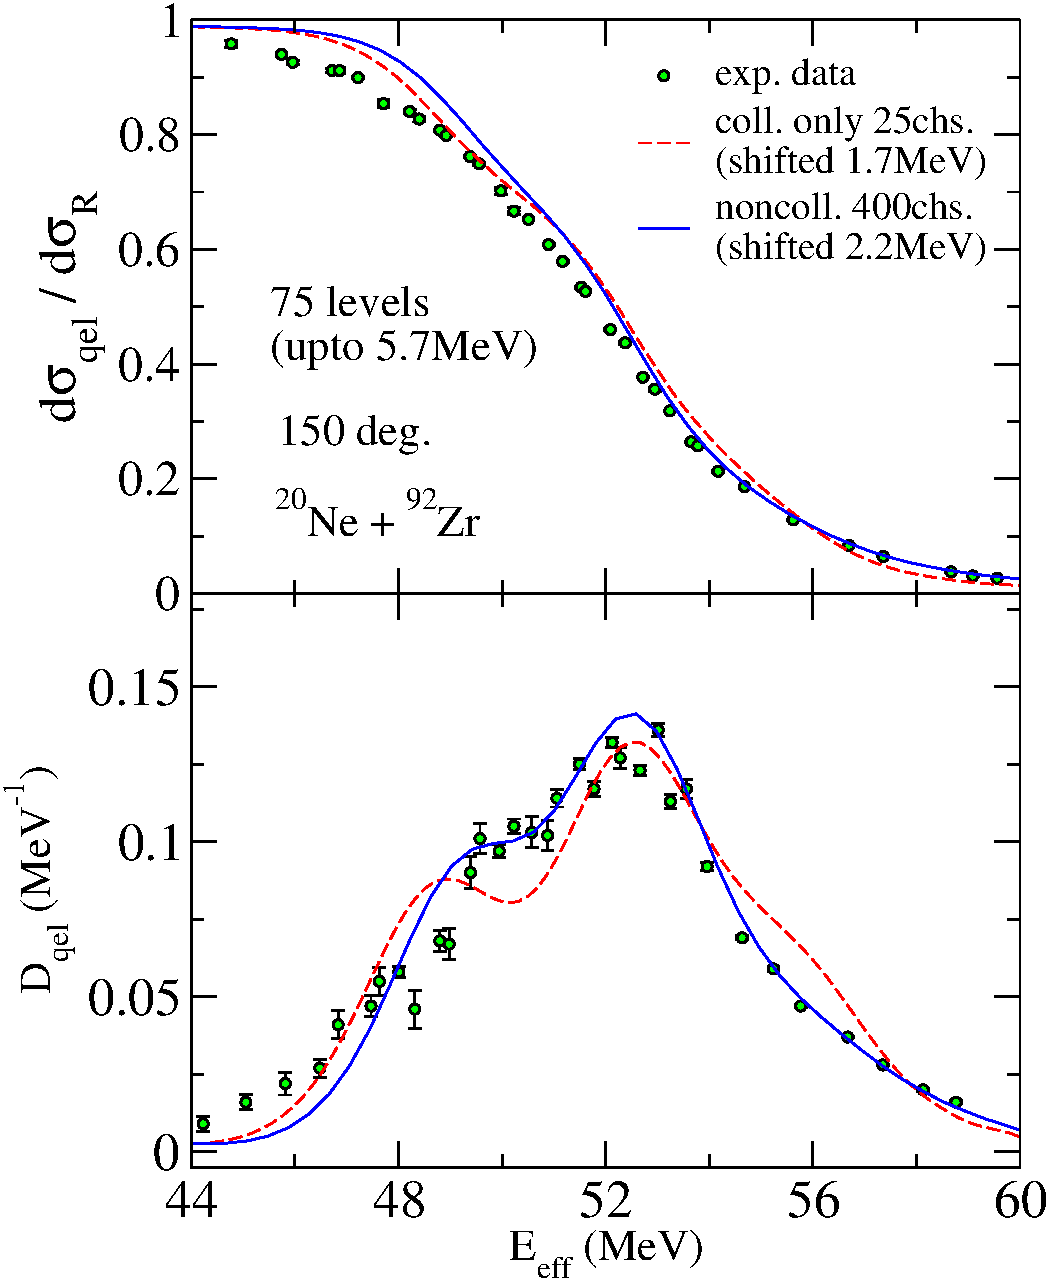
\includegraphics[clip,keepaspectratio,width=78mm]{figure/chapter7/qel_20Ne_92Zr_150deg_noncoll_w0_200_2.pdf}
    \caption{Same as Fig.\ref{fig7.9}, but for $^{20}$Ne + $^{92}$Zr system.}
    \label{fig7.10}
  \end{minipage}
\end{figure}
The same parameters are then used for the calculations for $^{20}$Ne + $^{90}$Zr
reaction.
The level density is constructed in the same way as that in the case of $^{16}$O +
$^{208}$Pb calculation, as we show in Figs. \ref{level_fit_90Zr} 
and \ref{ld_90Zr} for $^{90}$Zr and in Figs. \ref{level_fit_92Zr} and 
\ref{ld_92Zr} for $^{92}$Zr.
For $^{90}$Zr, $N(\epsilon)$ defined by Eq. (\ref{num_levels})
is fitted in the interval between 3 MeV and 8 MeV with a polynomial
$\displaystyle f(\epsilon) = \sum_{n=0}^{6}a_n \epsilon^n$.
The resultant parameters are
$a_0=199.2, a_1=182.5$ (MeV$^{-1}$), $a_2=-286.5$ (MeV$^{-2}$),
$a_3=119.7$ (MeV$^{-3}$), $a_4=-22.65$ (MeV$^{-4}$),
$a_5=2.057$ (MeV$^{-5}$), and $a_6=-0.07278$ (MeV$^{-6}$).
For $^{92}$Zr, $N(\epsilon)$ is fitted in the interval between
2.5 MeV and 6 MeV and the resultant parameters are
$a_0=63.79, a_1=540.7$ (MeV$^{-1}$), $a_2=-737.2$ (MeV$^{-2}$),
$a_3=366.7$ (MeV$^{-3}$), $a_4=-87.00$ (MeV$^{-4}$),
$a_5=10.07$ (MeV$^{-5}$), and $a_6=-0.4589$ (MeV$^{-6}$).
We take into account the mutual excitations of $^{20}$Ne and $^{90,92}$Zr.



\subsection{Results}
\subsubsection{Quasi-elastic scattering cross sections and barrier distribution}
\begin{figure}[t]
  \center
  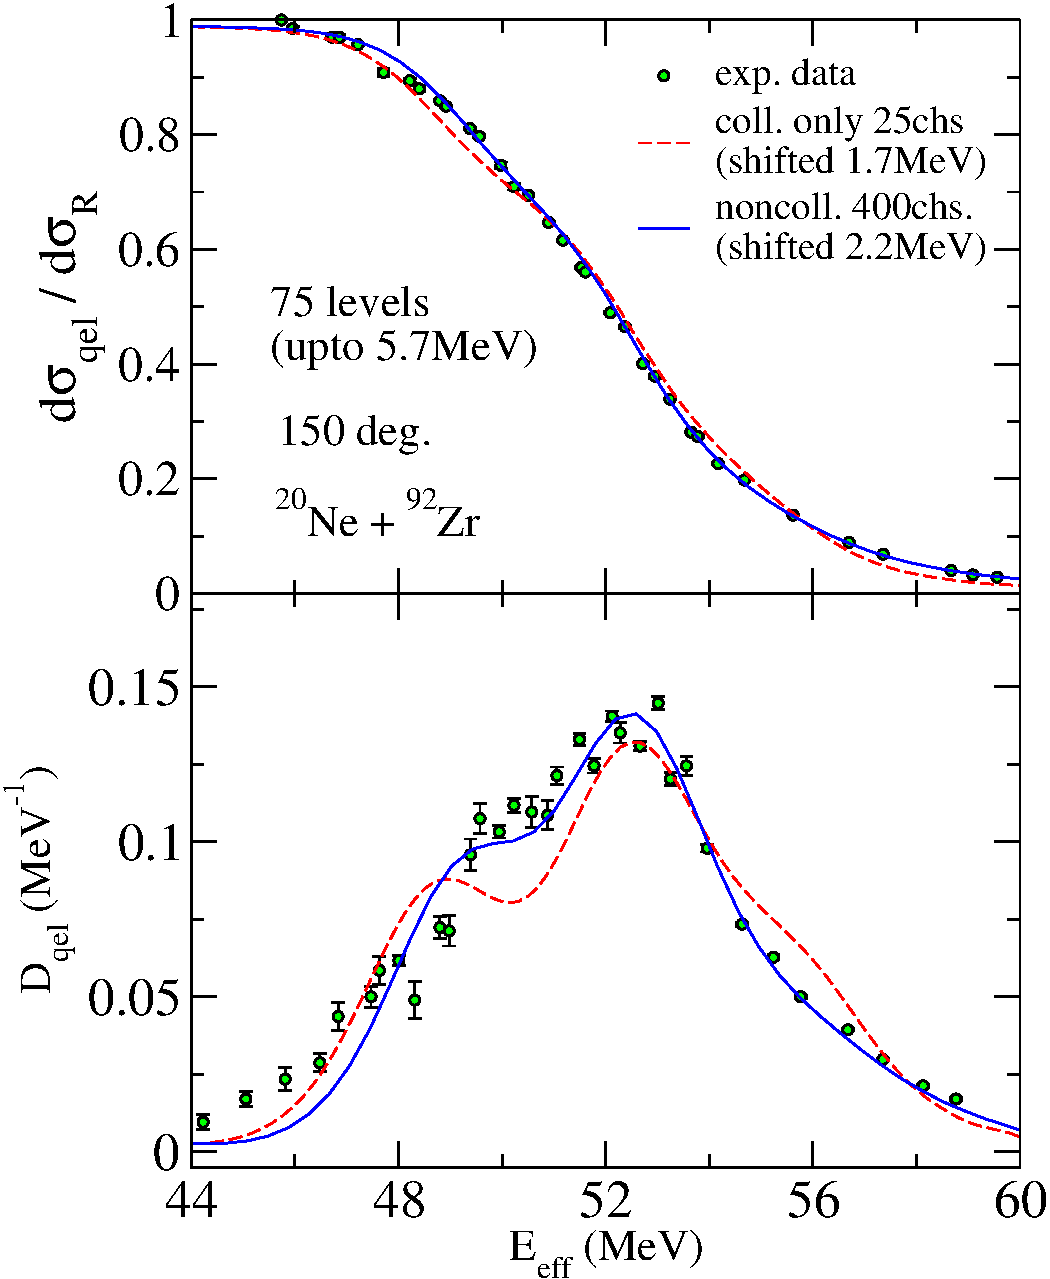
\includegraphics[clip,keepaspectratio,width=100mm]{figure/chapter7/qel_20Ne_92Zr_150deg_noncoll_w0_200_scaled_2.pdf}
  \caption{Same as Fig.\ref{fig7.10}, but with a scaling of
  the experimental data by a factor of 0.94.}
  \label{fig7.11}
\end{figure}

\begin{figure}[h]
  \center
  \begin{minipage}[t]{80mm}
    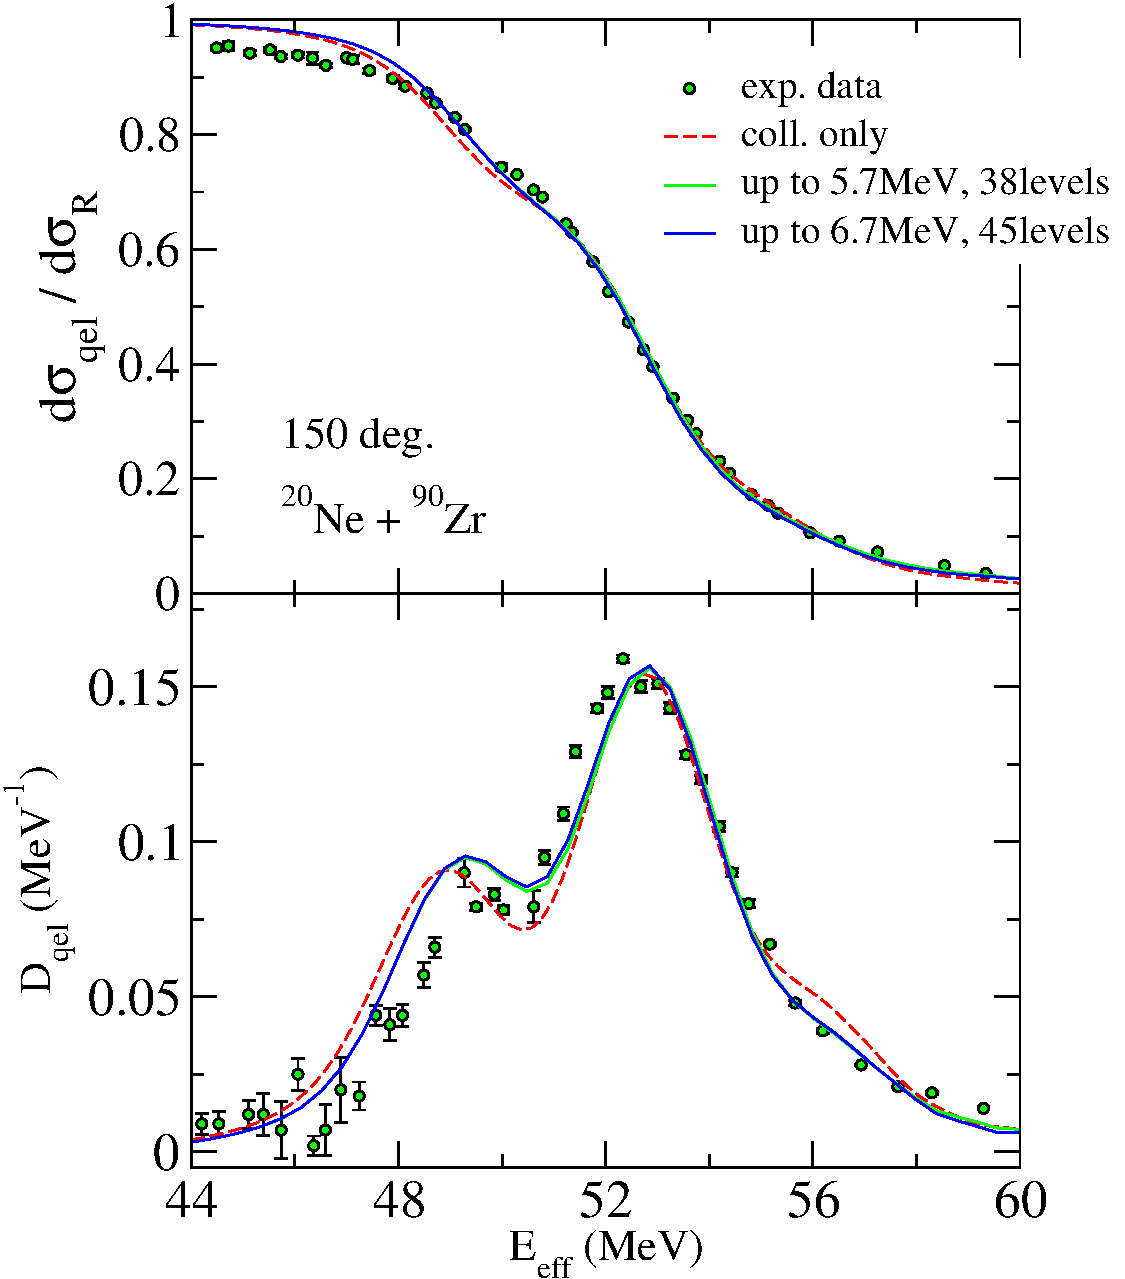
\includegraphics[clip,keepaspectratio,width=80mm]{figure/chapter7/qel_20Ne_90Zr_150deg_convergence_w0_200.pdf}
    \caption{Convergence of the coupled-channels calculation for $^{20}$Ne +
    $^{90}$Zr
    with respect to the truncation of excited states of
    $^{90}$Zr. The red dashed and the blue solid lines are the same as in
    Fig.\ref{fig7.9}. The green lines includes the noncollective levels up to 5.7 MeV.}
    \label{fig7.12}
  \end{minipage}
  \hspace{0.5cm}
  \begin{minipage}[t]{79mm}
    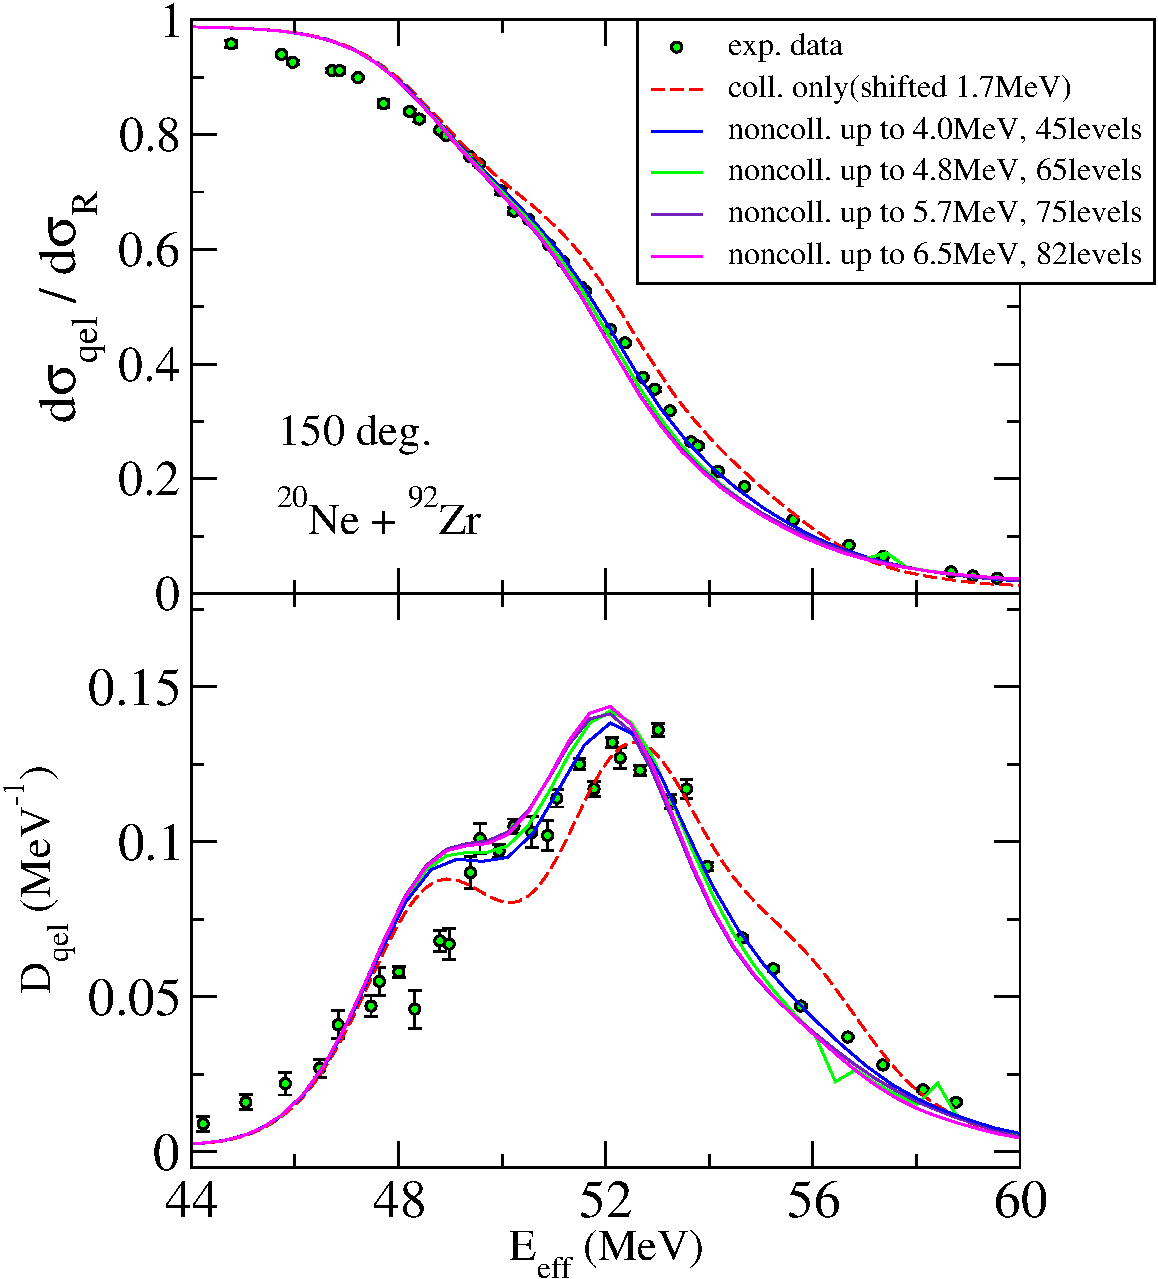
\includegraphics[clip,keepaspectratio,width=82mm]{figure/chapter7/qel_20Ne_92Zr_150deg_convergence_w0_200_2.pdf}
    \caption{Convergence of the coupled-channels calculation for $^{20}$Ne +
    $^{92}$Zr
    with respect to the truncation of excited states of
    $^{92}$Zr. The energy truncation is changed from 4.0 MeV to 6.5 MeV. The
    red dashed and the blue solid lines are the same as in Fig.\ref{fig7.10}.}
    \label{fig7.13}
  \end{minipage}
\end{figure}
We first show the results obtained by
including 45 noncollective levels in $^{90}$Zr nucleus
and 75 levels in $^{92}$Zr nucleus.
Inclusion of 45 noncollective levels corresponds to
taking into account excited states up to 6.7 MeV for $^{90}$Zr
and inclusion of 75 noncollective levels corresponds to 5.7 MeV for
$^{92}$Zr.
Figs.\ref{fig7.9} and \ref{fig7.10} show the quasi-elastic scattering cross
section and quasi-elastic barrier distribution for $^{20}$Ne + $^{90}$Zr and
$^{20}$Ne + $^{92}$Zr reactions, respectively.
For both figures, the dots represent the experimental data\cite{piasecki}
at the scattering angle $\theta_{\rm lab} = 150^\circ$,
the red dashed lines represent the results which take into account only the collective
excitations, and blue solid lines represent the results which take into account the
noncollective excitations in addition to the collective excitations.
In Figs.\ref{fig7.9}, \ref{fig7.10} 
the red and the blue lines are shifted in energy by 1.7 MeV
and 2.0 MeV, respectively, in order to adjust the barrier height.
The difference in the amount of shifts between the red dashed
line and the blue solid line originates from the potential renormalization due to the
high excitation energy of the noncollective states as has been discussed in the
reaction of $^{16}$O + $^{208}$Pb in the previous chapter.
For $^{20}$Ne + $^{90}$Zr reaction, we can see that even when we include the
noncollective excitations, they do not alter the barrier distribution
in a significant way with the
present parameters, although the
ditch between the two peaks is somewhat filled.
Thus, the noncollective excitations do not deteriorate the agreement with the
data for $^{20}$Ne + $^{90}$Zr quasi-elastic scattering.
On the other hand, for $^{20}$Ne + $^{92}$Zr reaction, the noncollective
excitations fill the ditch between the peaks and 
the peak structure is thus considerably smeared.
As a consequence, the agreement with the experimental barrier distribution is
much improved for the $^{20}$Ne + $^{92}$Zr system.
In these calculations, the same parameters in the random matrix model are used both
for $^{20}$Ne + $^{90}$Zr and $^{20}$Ne + $^{92}$Zr reactions.
Therefore, the difference of the effects of the noncollective
excitations comes from the level density in the form factor Eq. (\ref{goe_2})
and 
the level structure between $^{90}$Zr and $^{92}$Zr nuclei, that is, a
large number of noncollective states at a relatively low excitation energy region in
$^{92}$Zr .
We also notice that the agreement at the high energy tail of the
barrier distribution is also improved due to the noncollective excitations.

Although the barrier distributions are well reproduced by including the
noncollective excitations, the agreement of the 
quasi-elastic scattering cross sections becomes worse.
This may be due to the treatment of the normalization of the experimental cross sections.
In fact, if we divide the experimental data by 0.94,
the agreement for cross sections is improved
as is shown in Fig.
\ref{fig7.11} for the $^{20}$Ne + $^{92}$Zr system.
Notice that the shape of barrier distribution does not change by this
overall scaling.
In the experiment, the scattering cross sections are measured at a
forward angle($\theta_{\rm lab} = 35^\circ$) as well as backward angles.
Assuming the Rutherford cross sections for the measured cross sections
at the forward angle,
the corresponding scattering cross
sections at backward angles are obtained,
with which the experimental $\sigma_{\rm qel}/\sigma_{\rm R}$ is
constructed. The data is further normalized by setting the cross section to be
unity at the lowest incident energy in the measurement.
The data shown in Fig. \ref{fig7.11} correspond to those normalized at $E = 44$
MeV, rather than at the lowest energy.

\subsubsection{Convergence of calculated results}
We next discuss the convergence of the calculations 
with respect to the energy truncation.
\begin{figure}[t]
  \center
  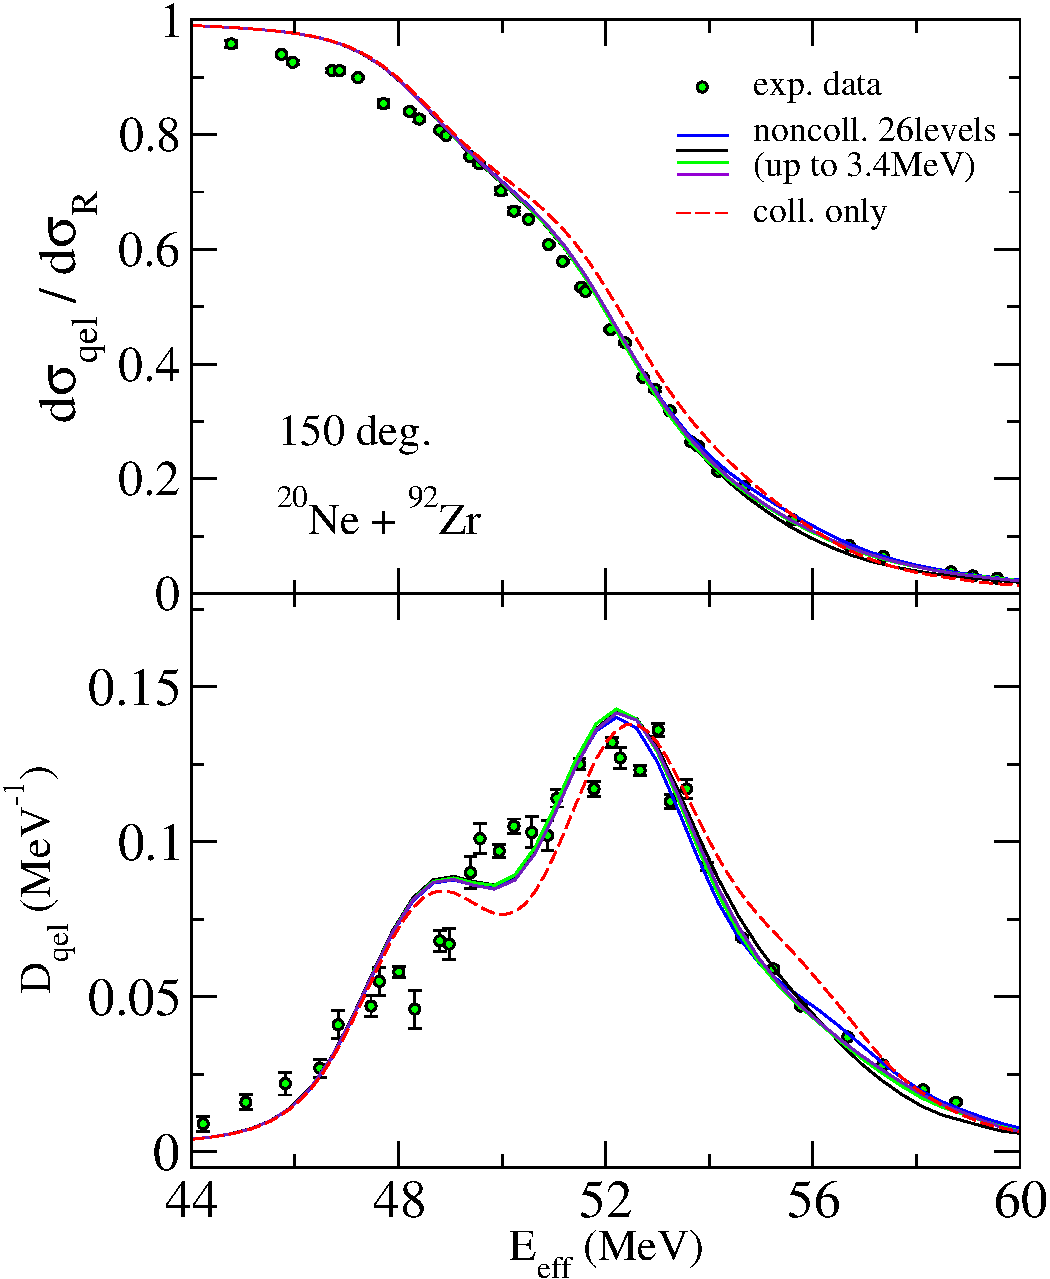
\includegraphics[clip,keepaspectratio,width=100mm]{figure/chapter7/qel_20Ne_92Zr_150deg_convergence_average_w0_200.pdf}
  \caption{Calculations with four differently generated coupling matrices in the random
  matrix model (the solid lines). The red dashed lines include only the collective
  excitations.}
  \label{fig7.14}
\end{figure}
In Fig.\ref{fig7.12}, we show the calculation for $^{20}$Ne + $^{90}$Zr
scattering. The red and the blue lines are the same as those in Fig.\ref{fig7.9}.
The green solid lines take into account the noncollective excitations up to
excitation energy 5.7 MeV, while up to 6.7 MeV for the blue lines.
The number of the noncollective levels up to 5.7 MeV is 38.
We can see that the green and the blue lines are almost the same, that is, 
the convergence is already obtained if one includes 38 levels for $^{90}$Zr
nucleus.
In Fig.\ref{fig7.13}, we show the calculation for $^{20}$Ne + $^{92}$Zr system
with several truncations of the noncollective excitations ranging from 4.0 MeV to 6.5
MeV. The red and the blue lines are the same as those in Fig.\ref{fig7.10}.
We can see the gradual increase of the effects of noncollective excitations and
that the convergence is obtained if one includes the excited states up to 5.7 MeV.
In Fig. \ref{fig7.13}, all the calculations are shifted by 1.7 MeV. 
We can see that the lower energy tail of the barrier distribution is hardly
altered by the noncollective excitations, while the higher region is shifted
towards the low-energy side.
We can understand this behavior from the energy dependence of the 
Q-value distribution discussed in the next subsection.

In the random matrix model, the meaningful quantity is the ensemble averaged
quantity.
The calculated results shown above are not ensemble averaged.
In order to see the dispersion due to the random matrix, we show in
Fig.\ref{fig7.14} the four calculations with differently generated coupling matrices
by the solid lines (these calculations take into account only 26 noncollective
levels in order to reduce the computational effort).
For comparison, we show the calculation with only the collective excitations by the red
dashed line. We can see that the dispersion due to the different random
matrices is sufficiently small compared to the change due to the noncollective
excitations.
This justifies the use of the non-averaged results in the discussion of
the noncollective effects.



\subsubsection{Q-value distribution}
We next present the calculation for a Q-value distribution in Figs.\ref{fig7.15}
and \ref{fig7.16} for $^{20}$Ne + $^{90}$Zr and $^{20}$Ne + $^{92}$Zr systems,
respectively.
\begin{figure}[t]
  \center
    \includegraphics[clip,keepaspectratio,width=120mm]{figure/chapter7/Qval_dist_90Zr_w0_200.eps}
    \caption{Q-value distributions for $^{20}$Ne + $^{90}$Zr system.
    The experimental data are
    taken at CM angle 156$^{\circ}$ and CM energy of 51.85 MeV\cite{piasecki}.
    The red dashed
    line includes only the collective excitations and the blue solid line
    includes the noncollective excitations as well.
    The calculations are taken at different energies corresponding to the 
    shift in the barrier distribution due to the potential renormalization.}
    \label{fig7.15}
\end{figure}
\begin{figure}[t]
  \center
    \includegraphics[clip,keepaspectratio,width=120mm]{figure/chapter7/Qval_dist_92Zr_w0_200_2.eps}
    \caption{Q-value distributions for $^{20}$Ne + $^{92}$Zr system. The meaning
    of each line is the same as Fig.\ref{fig7.15}.
    The experimental data are taken from Ref. \cite{piasecki-priv}.}
    \label{fig7.16}
\end{figure}
\begin{figure}[t]
  \center
    \includegraphics[clip,keepaspectratio,width=120mm]{figure/chapter7/Qval_dist_9092Zr_w0_200_2.eps}
    \caption{Comparison of the Q-value distributions between $^{20}$Ne + $^{92}$Zr
    and $^{20}$Ne + $^{92}$Zr systems.}
    \label{qdist_comp}
\end{figure}
In the figures, the dots represent the experimental data, the red dashed lines
represent the calculation with only the collective excitations and the blue 
solid lines represent the calculation with the noncollective excitations 
in addition to the collective excitations.
(The experimental data for $^{20}$Ne + $^{92}$Zr shown in Fig. 5 in
Ref. \cite{piasecki} has been found to be wrong\cite{piasecki-priv}.
The correct data are shown in Fig. \ref{fig7.16}.)
The experimental data are taken at $\theta_{\rm CM} = 156^{\circ}$ and
$E_{\rm CM} =51.85$ MeV and do not include the transfer processes.
The calculations shown in the figures are taken at different energies
corresponding to the shift in the barrier distribution due to the potential
renormalization.
These are smeared with a gaussian function Eq. (\ref{eq5.6}) with a
width of $\Delta = 0.5$ MeV to
adjust the width of the elastic peak of the data, 
and are normalized to the height
of the elastic peak.
We can see that in both systems, the noncollective excitations
have a small effect on the Q-value distribution at this incident energy.
For $^{20}$Ne + $^{90}$Zr system, the calculation reasonably
reproduces the data up to about 5 MeV, while above 5 MeV, it underestimates
the data.
For $^{20}$Ne + $^{92}$Zr system, 
the noncollective excitations enhance the contribution from the inelastic
channels between about 3 to 6 MeV, and the data is reasonably reproduced
up to 4 MeV.
Above 4 MeV, the present calculation
does not reproduce the data as in the case of $^{90}$Zr.
We compare the results of the two systems in Fig. \ref{qdist_comp}.
The blue ones are the experimental data and the calculation
for $^{20}$Ne + $^{90}$Zr system,
and the red ones are those for $^{20}$Ne + $^{92}$Zr system.
They are normalize at the height of the elastic peak.
We can see that the data show almost the 
same Q-value distribution between the two systems.
This suggests that the difference in the number of the 
noncollective states between $^{90}$Zr and $^{92}$Zr nuclei 
(see Fig. \ref{fig1.3})
does not affect the Q-value distribution at this energy.
This is consistent with our calculation show in the figure, and thus,
we conclude that our calculation accounts for the data
qualitatively well.

\begin{figure}[t]
  \center
    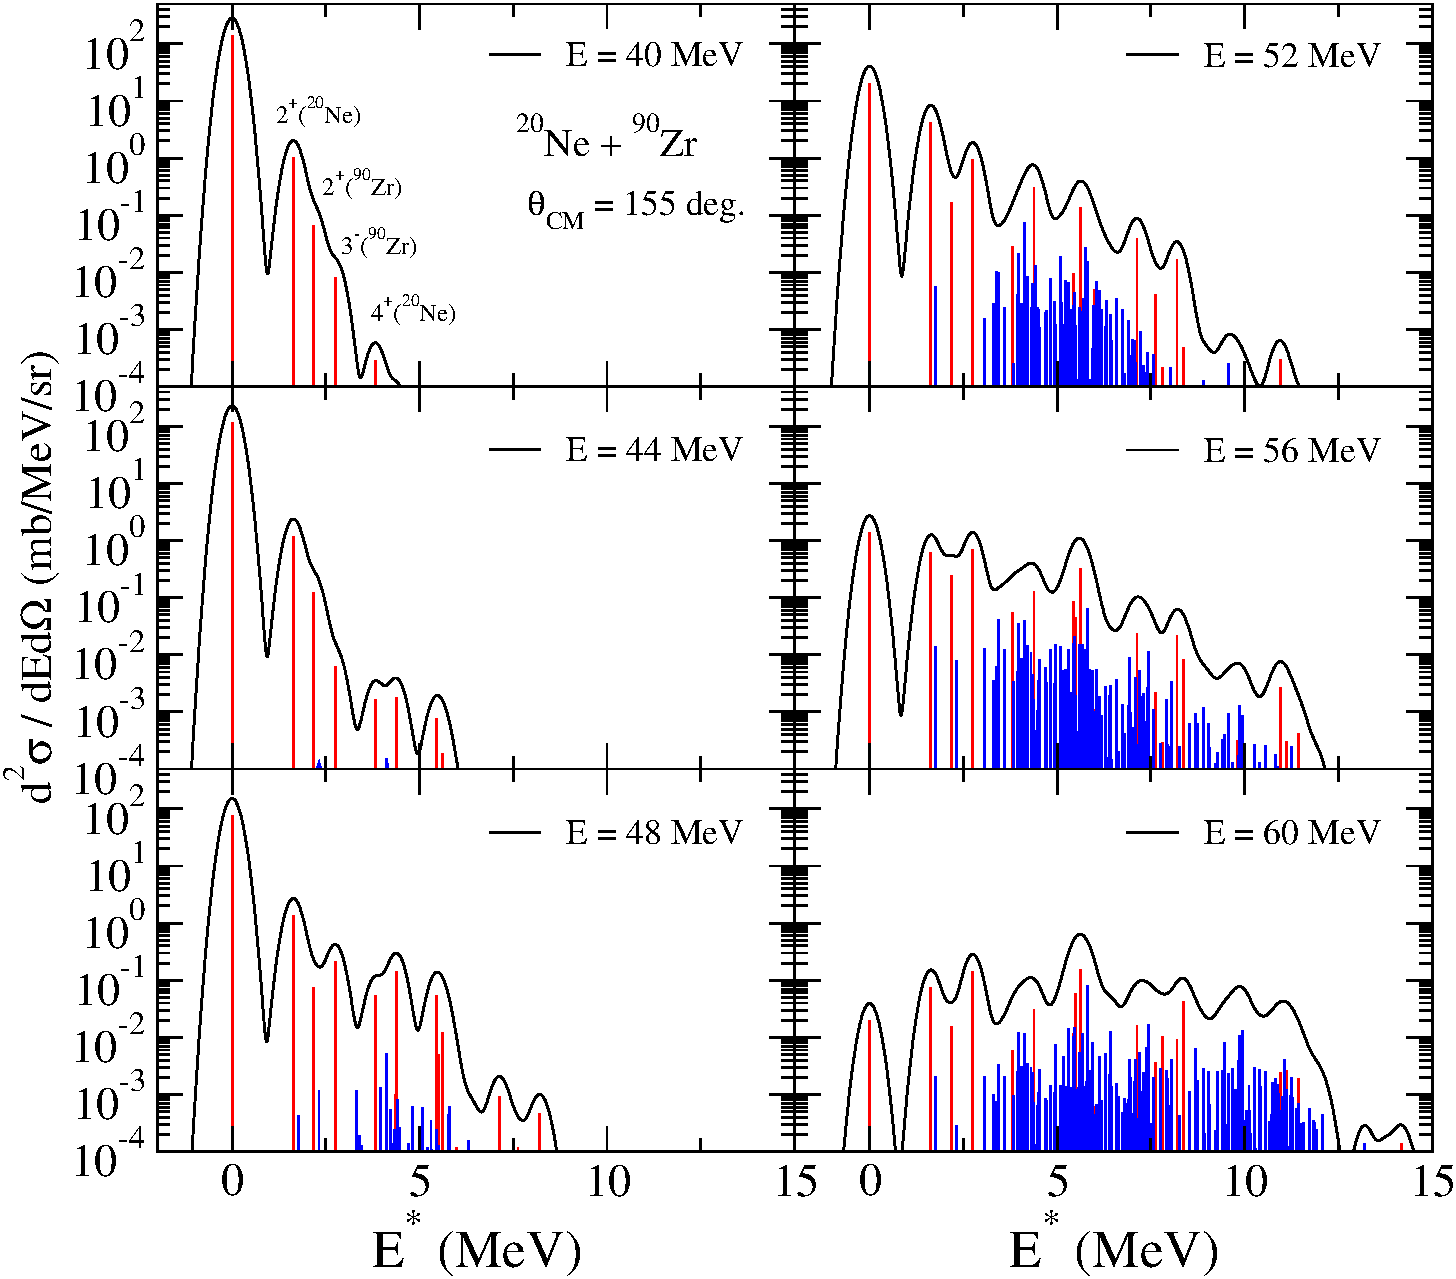
\includegraphics[clip,keepaspectratio,width=150mm]{figure/chapter7/Qval_dist_energy_dep_90Zr_w0_200.pdf}
    \caption{The energy dependence of the Q-value distribution for $^{20}$Ne +
    $^{90}$Zr system. The red and the
    blue spectra show the contribution from the collective and the
    noncollective channels, respectively. The black lines are obtained by
    smearing the spectra with a gaussian function with a width of 0.2 MeV.}
    \label{fig7.21}
\end{figure}
However, this does not mean that the noncollective excitations are not important
in the Q-value distribution.
We have seen that the contribution from the noncollective excitation becomes
important as the incident energy increases for the reaction of $^{16}$O +
$^{208}$Pb system.
In fact, the same tendency is observed
for $^{20}$Ne + $^{90,92}$Zr systems as shown in Figs.
\ref{fig7.21} and \ref{fig7.22}.
These figures show the Q-value distribution at different incident energies
from 40 MeV to 60 MeV. The solid red spectra show the contribution from the
collective channels, the blue spectra show the contribution from the
noncollective channels, and the envelope shows the Q-value distribution
smeared with a gaussian function with a width of 0.2 MeV.
For both systems, the contribution from the collective excitations is dominant
below the barrier (about 52 MeV), while the contribution from the noncollective
excitations becomes important as the incident energy increases.
However, the peak structure of the Q-value distribution is mainly constructed by
the collective excitations for $^{20}$Ne + $^{90}$Zr system even above the
Coulomb barrier. On the other hand,
for $^{20}$Ne + $^{92}$Zr system, the noncollective
excitations also contribute to the
construction of a peak structure.
Since the contribution from the noncollective excitations
is important at larger (above barrier) energies, the potential
renormalization can be observed in the high energy region in Fig. \ref{fig7.13}.

\begin{figure}[t]
  \center
    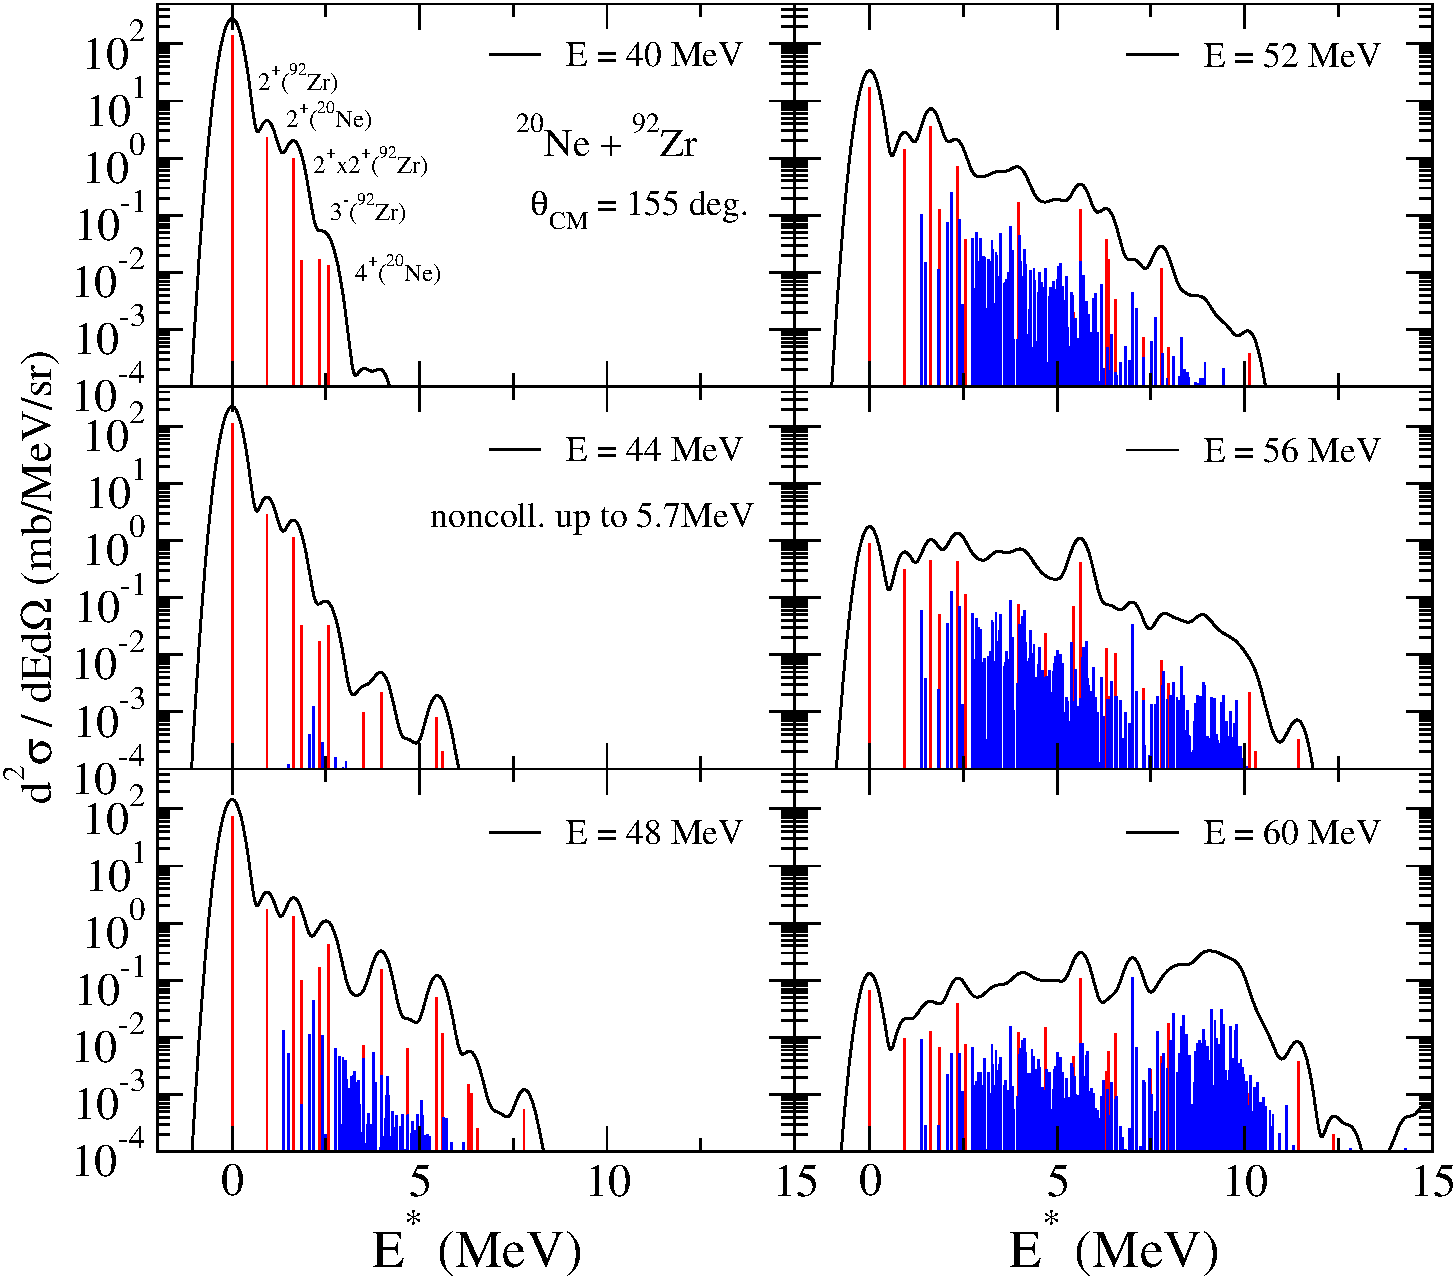
\includegraphics[clip,keepaspectratio,width=150mm]{figure/chapter7/Qval_dist_energy_dep_92Zr_w0_200_2.pdf}
    \caption{Same as Fig.\ref{fig7.21}, but for $^{20}$Ne + $^{92}$Zr system.}
    \label{fig7.22}
\end{figure}
In order to observe the effect of the noncollective excitations on the Q-value
distribution, it will be necessary to measure the data above 
the barrier energies and see the energy dependence.

\subsubsection{Reactions with different projectiles}
We have shown that the
noncollective excitations of $^{90,92}$Zr nuclei improve the
calculations for $^{20}$Ne + $^{90,92}$Zr reactions.
In order to see whether our description
of the noncollective excitations works for
other reactions, we apply the model to $^{16}$O + $^{92}$Zr and
$^{28}$Si + $^{92}$Zr fusion reactions, where the fusion cross sections
are experimentally obtained and coupled-channels analyses have
been performed\cite{NMD01}.
\begin{figure}[t]
  \center
  \begin{minipage}[t]{80.2mm}
    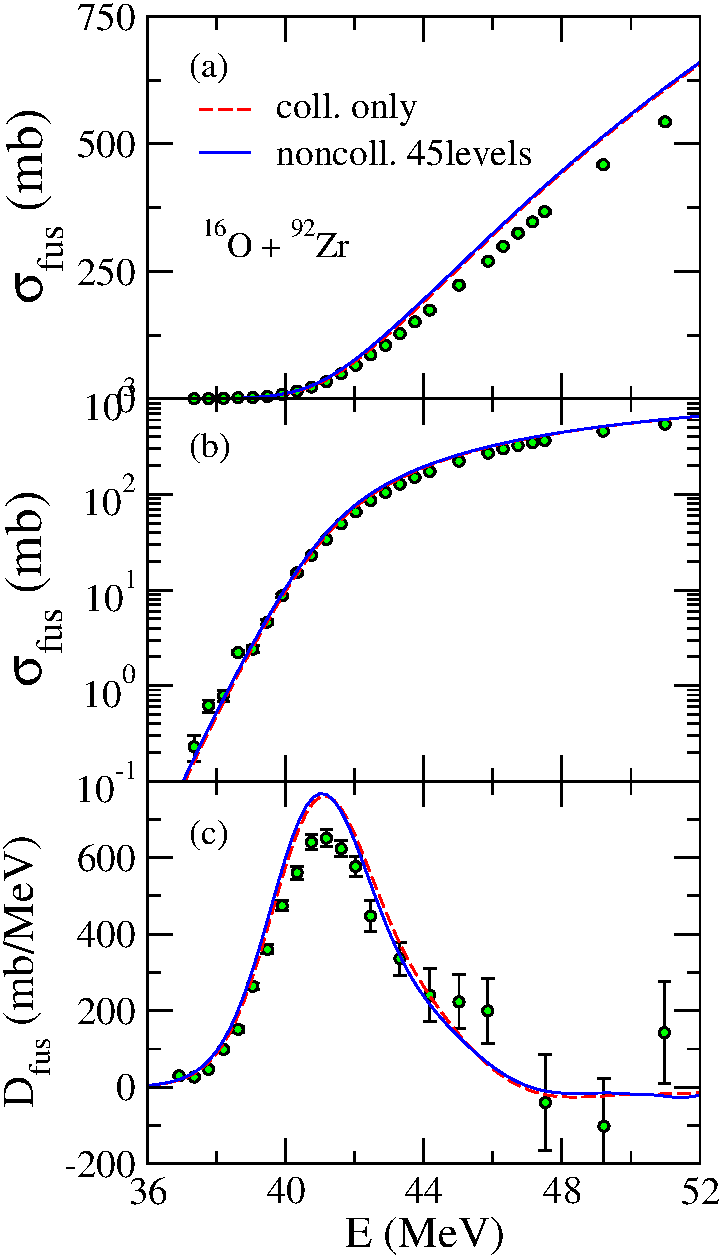
\includegraphics[clip,keepaspectratio,width=80.2mm]{figure/chapter7/fus_16O_92Zr_noncoll_w0_200.pdf}
    \caption{Fusion cross sections and the fusion barrier distribution for
    $^{16}$O + $^{92}$Zr system. The meaning of each line is the same as in the
    calculation for $^{20}$Ne + $^{92}$Zr system. The experimental data are
    taken from Ref. \cite{NMD01}.}
    \label{fig7.17}
  \end{minipage}
  \hspace{0.5cm}
  \begin{minipage}[t]{78.5mm}
    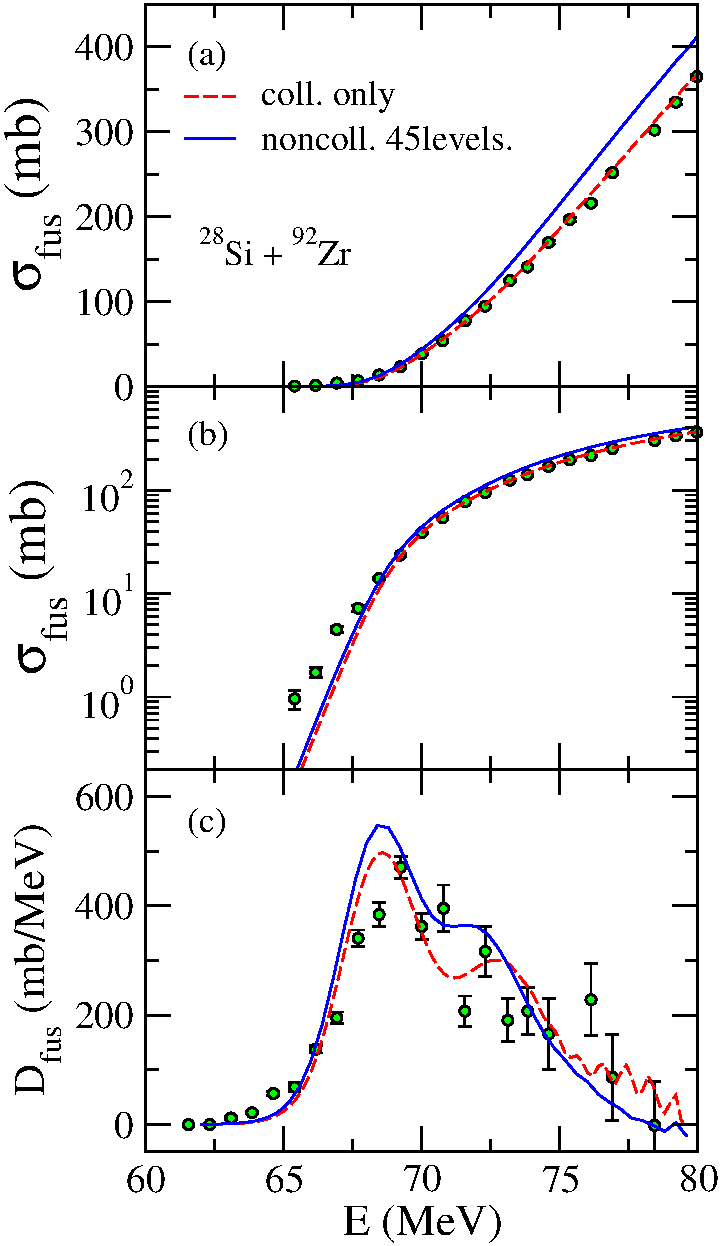
\includegraphics[clip,keepaspectratio,width=78.5mm]{figure/chapter7/fus_28Si_92Zr_noncoll_w0_200.pdf}
    \caption{Same as Fig.\ref{fig7.17}, but for $^{28}$Si + $^{92}$Zr
    system. The experimental data are taken from Ref. \cite{NMD01}.}
    \label{fig7.18}
  \end{minipage}
\end{figure}
Figs.\ref{fig7.17} and \ref{fig7.18} show the results for
$^{16}$O + $^{92}$Zr and $^{28}$Si + $^{92}$Zr systems, respectively.
In both figures, the dots represent the experimental data\cite{NMD01},
the red lines represent
the calculation with only the collective excitations, and the blue lines represent
the calculation with the noncollective excitations in addition to the collective
excitations. The upper and the middle panels show the fusion cross sections in
the linear and logarithmic scales, respectively,
while the bottom panel shows the
fusion barrier distribution.
For the $^{16}$O projectile,
we take into account the vibrational $3^-$ state at 6.13 MeV as in the
reaction for $^{16}$O + $^{208}$Pb system discussed in the previous chapter.
The potential parameters in the Woods-Saxon potential are $V_0 = 55.16$ MeV for
the potential depth, 
$r_0=1.17$ fm for the radius parameter, and $a = 0.60$ fm for the surface
diffuseness parameter. These parameters are chosen so that the calculation
reproduces the height of the Coulomb barrier.
We can see that the noncollective excitations hardly affect the barrier
distribution.
For this system, the barrier distribution has almost a 
single peak structure even in
the absence of the noncollective excitations.
This is because the vibrational excitations of $^{92}$Zr are not so strong to yield
a well structured barrier distribution and the octupole phonon state in $^{16}$O
only renormalizes the potential barrier.
Therefore, the smearing due to
the noncollective excitations does not change the shape of the barrier
structure.
In addition to this, the smaller charge product of of the projectile and the target
also makes the effect
of the noncollective excitations small compared to that in the $^{20}$Ne +
$^{92}$Zr system.

For the $^{28}$Si projectile, we take into account the rotational excitations with
$\epsilon_2 = 1.779$ MeV and $\beta_2 = -0.407$ up to the $6^+$ state, and the
octupole one-phonon state with $\epsilon_3 = 6.88$ MeV and $\beta_3 =0.280$.
The potential parameters in the Woods-Saxon potential are
$V_0=60.25$ MeV, $r_0 = 1.18$ fm, and $a = 0.63$ fm.
We can see that the barrier distribution is smeared due to the
noncollective excitations and the peak structure becomes unclear.
%The magnitude of the noncollective effect is larger than that in the $^{20}$Ne +
%$^{92}$Zr system. This is due to the larger charge product for this system.
%While the agreement with the data seems to be slightly worsened due to the
%noncollective excitations,
This calculation is also consistent with the data,
although it is not clear whether the non-collective excitations
lead to an improvement due to the large error bars.
The slope of the fusion cross sections at energies 
above the barrier becomes steeper by
the noncollective excitations and the agreement with the data is worsened.
However, this is not a serious problem because
one can adjust the surface diffuseness parameter $a$ in the
nuclear potential so that the slope is consistent with the experimental data. 

We have also performed a 
coupled-channels calculation for $^{28}$Si + $^{90}$Zr system to see the effect
of the noncollective excitations of $^{90}$Zr in different system.
We have found that the noncollective excitations of $^{90}$Zr nucleus 
have a minor effect on the barrier distribution as in the case of
$^{20}$Ne +$^{90}$Zr scattering. That is, it smears the peak structure of the
barrier distribution only slightly.

From these considerations, we argue that the noncollective excitations described in
this model does not lead to an inconsistency with the previous analyses for the
systems studied in this subsection.

In this subsection, we have investigated the effect of the noncollective
excitations in systems with different projectiles. We have seen that,
depending on the type of the collective excitations in the projectile, the
noncollective excitations affect the barrier distribution in a different way.
In App. D, we present the study of the interplay of the collective and the noncollective
excitations using a schematic model.
This study shows that the noncollective excitations tend to shrink the distance
between peaks of the barrier distribution, if the collective excitations, which
dominates the barrier structure, are rotational excitations associated with
a prolate deformation.


\section{Prediction for $^{24}$Mg + $^{90,92}$Zr reaction}
Before we close this chapter, 
we present the theoretical prediction for $^{24}$Mg
+ $^{90,92}$Zr reactions.
The reason why we choose this system is that the 
$^{24}$Mg is a strongly deformed nucleus with
prolate shape ($\beta_2 = 0.505$) and thus the similar noncollective
effect on the barrier distribution can be expected
as in the $^{20}$Ne + $^{90,92}$Zr system.
In Figs.\ref{fig7.19} and \ref{fig7.20}, we show the fusion calculation for
$^{24}$Mg + $^{90,92}$Zr systems.
The meaning of the red dashed lines and the 
blue solid lines is the same as in Fig. \ref{fig7.9}.
For the coupling to $^{24}$Mg nucleus, 
we include the rotational states up to 6$^+$ state.
For the nuclear potential, we use the Aky\"{u}z-Winther
potential\cite{Akyuz-Winther}.
In the presence of only the collective excitations, the barrier
distributions for the $^{24}$Mg + $^{90,92}$Zr systems exhibit similar behavior 
to those for the $^{20}$Ne + $^{90,92}$Zr systems. 
We can see that for $^{24}$Mg + $^{90}$Zr reaction, the effect of the
noncollective excitations is not significantly large.
It steepens the shoulder of the high energy
part of the barrier distribution and fills the dip around 59 MeV.
On the other hand, the noncollective excitations drastically change the behavior
of the barrier distribution for $^{24}$Mg + $^{92}$Zr system. The effect of the
noncollective excitations is similar to that in the $^{20}$Ne + $^{92}$Zr
system, but stronger.
This is because the charge product of $^{24}$Mg + $^{92}$Zr system and 
the deformation parameter $\beta_2$ of the projectile are larger
than those of $^{20}$Ne + $^{92}$Zr system.
If the fusion or quasi-elastic barrier distribution was measured for
this system and the smeared structure was found for $^{24}$Mg +
$^{92}$Zr system, the validity of our scenario would become clearer.
However, the transfer processes may affect the barrier distribution for
$^{24}$Mg + $^{90,92}$Zr differently, and in that case
one should consider their effects as well.
\begin{figure}[t]
  \center
  \begin{minipage}[t]{78mm}
    \includegraphics[clip,keepaspectratio,width=78mm]{figure/chapter7/fus_24Mg_90Zr_noncoll_w0_200.eps}
    \caption{Fusion cross sections and fusion barrier distribution for
    $^{24}$Mg + $^{90}$Zr system. The meaning of each line is the same as in
    Fig.\ref{fig7.9}.}
    \label{fig7.19}
  \end{minipage}
  \hspace{0.5cm}
  \begin{minipage}[t]{78mm}
    \includegraphics[clip,keepaspectratio,width=78mm]{figure/chapter7/fus_24Mg_92Zr_noncoll_w0_200.eps}
    \caption{Same as Fig.\ref{fig7.19}, but for $^{24}$Mg + $^{92}$Zr system.}
    \label{fig7.20}
  \end{minipage}
\end{figure}


\end{document}

